% Map of the agent rules in Config/.cursor/rules, grouped by when they load.
% Build: latex-scientific rule, "TikZ figures: SVG first, PDF last".
\documentclass[border=6pt]{standalone}
\usepackage{amsmath}
\usepackage{fontspec}
\usepackage{unicode-math}
\setmathfont{STIX Two Math}
\setmainfont{TeX Gyre Heros}[Ligatures=CommonOff] % ligature glyphs have no Unicode in the SVG
\usepackage{xcolor}
\usepackage{tikz}
\usetikzlibrary{positioning,fit,calc,backgrounds}
\hyphenpenalty=10000
\exhyphenpenalty=10000

\definecolor{ink}{HTML}{1C2B24}
\definecolor{green}{HTML}{0E4D3A}
\definecolor{blue}{HTML}{1D4E89}
\definecolor{orange}{HTML}{C45C26}
\definecolor{paper}{HTML}{F6F3EE}
\definecolor{grid}{HTML}{D9D3C7}

\tikzset{
  every node/.style={text=ink},
  rule/.style={draw=#1, line width=0.8pt, rounded corners=3pt, fill=white,
    text width=52mm, inner sep=2.4mm, align=left, font=\small},
  rule/.default=blue,
  group/.style={draw=grid, line width=0.8pt, rounded corners=6pt,
    fill=paper, inner sep=3.5mm},
  gtitle/.style={font=\bfseries, text=green, anchor=south west, inner sep=1mm},
  trig/.style={font=\footnotesize\itshape, text=ink!70, anchor=south east,
    inner sep=1mm},
}
% \R{name}{role}: rule box text
\newcommand{\R}[2]{\textbf{#1}\\[0.5mm]{\footnotesize #2}}

\begin{document}
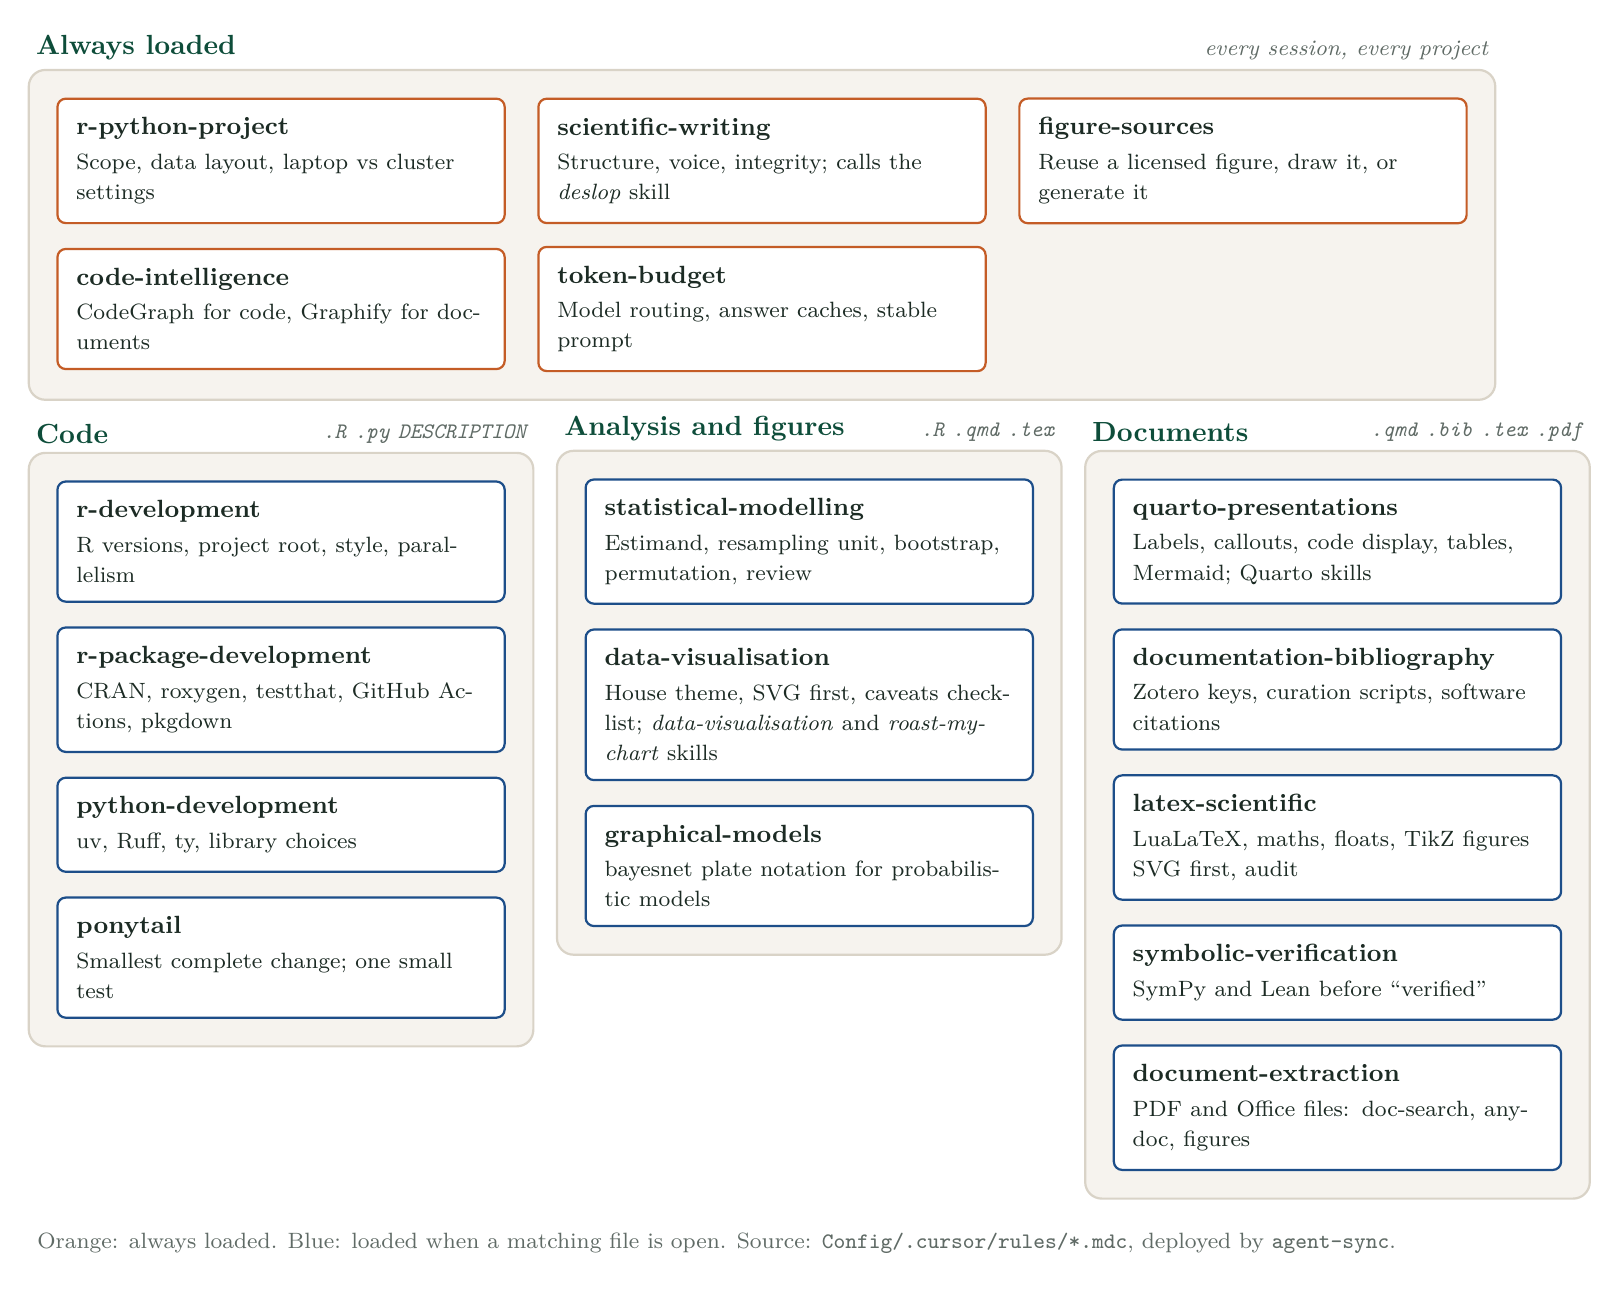
\begin{tikzpicture}[node distance=3mm and 4mm]

% ---- Always loaded ------------------------------------------------------
\node[rule=orange] (scope) {\R{r-python-project}{Scope, data layout, laptop vs cluster settings}};
\node[rule=orange, right=of scope] (write) {\R{scientific-writing}{Structure, voice, integrity; calls the \textit{deslop} skill}};
\node[rule=orange, right=of write] (figsrc) {\R{figure-sources}{Reuse a licensed figure, draw it, or generate it}};
\node[rule=orange, below=of scope] (code) {\R{code-intelligence}{CodeGraph for code, Graphify for documents}};
\node[rule=orange, right=of code] (budget) {\R{token-budget}{Model routing, answer caches, stable prompt}};
\begin{scope}[on background layer]
  \node[group, fit=(scope)(write)(figsrc)(code)(budget)] (always) {};
\end{scope}
\node[gtitle] at (always.north west) {Always loaded};
\node[trig] at (always.north east) {every session, every project};

% ---- R and Python -------------------------------------------------------
\node[rule, below=14mm of code] (rdev) {\R{r-development}{R versions, project root, style, parallelism}};
\node[rule, below=of rdev] (rpkg) {\R{r-package-development}{CRAN, roxygen, testthat, GitHub Actions, pkgdown}};
\node[rule, below=of rpkg] (py) {\R{python-development}{uv, Ruff, ty, library choices}};
\node[rule, below=of py] (pony) {\R{ponytail}{Smallest complete change; one small test}};
\begin{scope}[on background layer]
  \node[group, fit=(rdev)(rpkg)(py)(pony)] (code-g) {};
\end{scope}
\node[gtitle] at (code-g.north west) {Code};
\node[trig] at (code-g.north east) {\texttt{.R} \texttt{.py} \texttt{DESCRIPTION}};

% ---- Analysis and figures -----------------------------------------------
\node[rule, right=10mm of rdev] (stats) {\R{statistical-modelling}{Estimand, resampling unit, bootstrap, permutation, review}};
\node[rule, below=of stats] (dataviz) {\R{data-visualisation}{House theme, SVG first, caveats checklist; \textit{data-visualisation} and \textit{roast-my-chart} skills}};
\node[rule, below=of dataviz] (pgm) {\R{graphical-models}{bayesnet plate notation for probabilistic models}};
\begin{scope}[on background layer]
  \node[group, fit=(stats)(dataviz)(pgm)] (fig-g) {};
\end{scope}
\node[gtitle] at (fig-g.north west) {Analysis and figures};
\node[trig] at (fig-g.north east) {\texttt{.R} \texttt{.qmd} \texttt{.tex}};

% ---- Documents ----------------------------------------------------------
\node[rule, right=10mm of stats] (quarto) {\R{quarto-presentations}{Labels, callouts, code display, tables, Mermaid; Quarto skills}};
\node[rule, below=of quarto] (bib) {\R{documentation-bibliography}{Zotero keys, curation scripts, software citations}};
\node[rule, below=of bib] (latex) {\R{latex-scientific}{LuaLaTeX, maths, floats, TikZ figures SVG first, audit}};
\node[rule, below=of latex] (sym) {\R{symbolic-verification}{SymPy and Lean before ``verified''}};
\node[rule, below=of sym] (extract) {\R{document-extraction}{PDF and Office files: doc-search, anydoc, figures}};
\begin{scope}[on background layer]
  \node[group, fit=(quarto)(bib)(latex)(sym)(extract)] (doc-g) {};
\end{scope}
\node[gtitle] at (doc-g.north west) {Documents};
\node[trig] at (doc-g.north east) {\texttt{.qmd} \texttt{.bib} \texttt{.tex} \texttt{.pdf}};

\node[font=\footnotesize, text=ink!70, anchor=north west, align=left]
  at ($(code-g.west |- doc-g.south)+(0,-3mm)$)
  {Orange: always loaded. Blue: loaded when a matching file is open.
   Source: \texttt{Config/.cursor/rules/*.mdc}, deployed by \texttt{agent-sync}.};
\end{tikzpicture}
\end{document}
